\chapter{Background}\label{ch:background}

Modularity in programming dates back at least to Parnas and his
information hiding criteria\cite{parnas72}. There are two main lines
in the development of module systems. First, the Modula
\cite{wirth:module} and Cedar/Mesa \cite{cacm:mesa} line emphasized
{\it ad hoc} and extralinguistic schemes for modeling linking of
program modules,\ie, such languages used a separate tool, an object
file format sensitive link-loader, to compose separately compiled
modules.  Second, the ML line of modularity
\cite{macqueen:lfp84,macqueen:popl86,macqueen:lfp88} described
modularity in terms of a small functional programming language where
application is the main linkage mechanism. Common to both of these approaches is the idea that the separation of interface and implementation leads to better program structure. 

The original motivation for program modularity was highly pragmatic. Computers with very small main memory could not compile a large program efficiently because program source could not fit into memory all at once. Early languages partitioned programs into separate compilation units so that each individual compilation unit can mostly fit into memory and therefore be amenable to efficient compilation. As machine architecture progresses, program modularity is of increasing importance. Because most compiler optimization techniques rely on delicate data and control flow information and thus are sequential, modern compilers are rarely parallelized beyond the compilation of program modules in parallel. Compilers such as distcc can only take advantage of multiple cores during compilation if programs are broken down into finely separated compilation units. Thus, modularity is necessary for efficient compilation even on modern architectures. 


Modules in ML may include type components. This provision affords the programmer considerable power and fine-grain control. The ML module system serves three main functions:
\begin{enumerate}
	\item hierarchically organizes source (namespace management)
	\begin{lstlisting}
structure A =
struct
  structure B = 
  struct 
    structure C = struct type t = int end 
  end 
  type u = unit
end		
	\end{lstlisting}
	\item provides a mechanism for generic programming through parameterization
\begin{lstlisting}
functor F(X:sig type t end) =
struct
  type u = X.t 
end	
\end{lstlisting}
	\item enforces abstraction boundaries
\begin{lstlisting}
structure M = struct type secret = int end :> sig type secret end	
\end{lstlisting}
\end{enumerate} 

The most basic form of modularity is namespace management. Simple namespace management only requires a means to declare namespaces at the top-level of program structure (namespace N), functions that reside inside those namespaces, and a notation for accessing members of one namespace from another (N.f). Each namespace is a module in such a system. One can neither manipulate nor reference a namespace outside of the projection notation. A programmer can call functions by projecting out the desired components from these rudimentary modules. Namespace management, however, is only a convenience for the programmer. It provides no additional expressiveness or power in the language. In particular, namespace management by itself does not support separate compilation, which is crucial for independent development of components of a large software project and efficient compilation. In fact, without separate compilation, some programs would have been impossible to compile with the limited resources on early machines. Even on modern machines, large software compilation can be quite taxing. Many languages did not gain even a rudimentary module system until the late 1980s and early 1990s. For example, the venerable FORTRAN did not include a rudimentary module system until FORTRAN 90. 

A record of functions and variables can be used as a slightly richer form of modularity. In functional languages, regular records may also contain functions as fields. Records aggregate labeled fields that can be projected. Unlike namespaces, records are typically first-class, so functions on records enable a degree of generic programming especially in conjunction with row polymorphism~\cite{remy:popl89}. Unfortunately, records normally do not support data abstraction. Pierce's model of object-oriented languages uses records as its core construct~\cite{Pierce:TypeSystems}. Lampson and Burstall's Pebble language featured heterogeneous records that contained both values and types~\cite{lampsonburstall88}. Cardelli's Quest and Fun languages couple System F-like languages with heterogeneous records~\cite{cardelli:tp}. 

\section{Module Systems in Other Languages}
Modula-2 pioneered many of the major ideas behind module systems. It supported hierarchical composition (\ie, nesting), type components, and an exception handling mechanism~\cite{wirth:module}. The exception handling mechanism consisted of exception declarations as components of modules and a module-level exception handler. Compositions of modules were limited to explicit imports and exports of definite modules (as in a specific concrete module with all its components filled out) and their components. 

Ada is an example of an imperative and object-oriented language that supports modularity in the form of basic and generic packages \cite{bray:impl}. Packages are specified in two parts, specifications (akin to interfaces or signatures) and bodies which define the implementation of the package. Generic packages map basic packages to basic packages, thus provide a form of parameterization. Basic packages can be nested. Ada supports type components in modules (called packages) and ``generic'' modules parameterized on a single restricted type and some associated operator definitions. 

Object-oriented languages use the class or object system to provide a degree of modularity for functions and data. Most object-oriented languages with the exception of Scala~\cite{odersky-et-al:ecoop03} do not support type components, thus limiting their expressiveness. Scala's object system supports type components as members of a class. Beyond simple namespace management, OO languages support information hiding via private data members. Unlike in ML module systems, information hiding is achieved by annotating member fields and functions with a label private or protected instead of hiding type definitions. Unfortunately, this is a rather coarse-grain encoding even with multiple levels of privacy, visibility to an external client is all-or-nothing. Scala's structured types offer another approach to modularity. There has also been a considerable amount of interest in Bracha's mixin approach to modularity \cite{brachacook:mixin,bracha:thesis,duggan96} and traits \cite{Scharli03traits:composable,typed-traits-tr}. 

		Type classes~\cite{wadlerblott} can be modeled using a very stylized form of modules coupled with a dictionary-passing type inference~\cite{dhck07}. Where type classes apply, this inference scheme makes code significantly more succinct. However, as the set of instances of classes at any one point in the program is global, type classes sometimes interfere with modular programming. 
		
\section{The ML Module System}
The ML module system consists of structures, signatures, functors (parameterized modules), and functor signatures. Structures are sequences of type, value, structure, and functor bindings. In Standard ML, structures can be named or anonymous. Signatures are sets of specifications for types, the types of values, structure component signatures, and functor component signatures. Similar to structures, signatures can be either named and anonymous. Anonymous signatures are either written inline (\ie, \lstinline{sig ... end}) or extracted (inferred) from a structure. There is a many-to-many relationship between structures and signatures. Ascribing a signature to a structure verifies that that structure satisfies the signature. Alternatively, one can use a signature $SIG$ to seal a structure $M$ which hides or reveals type definitions selectively as required by $SIG$. Type specifications in signatures can be transparent definitions (\lstinline{type t = unit}), open  (\lstinline{type u}), or translucent specs defined relative to open specs (\lstinline{type v = u * int}), usually considered a kind of transparent specification. 

The module system of ML can express much of System F. Indeed, the SML/NJ compiler compiles source into a System F-like core language (see chapter~\ref{ch:translation}). Although the Definition\cite{mthm97} does not require nor define support for higher-order modules, they can be found in many implementations of Standard ML including SML/NJ, Moscow ML, and MLton. Higher-order module systems are not found outside of the ML family of module systems. Functors can be typechecked independently from their uses (\ie, applications) unlike related programming constructs such as C++ templates. Separate typechecking is necessary for true independent development of large software systems. It also makes it possible to gain confidence in the type safety of the functor before even beginning to write functor arguments and applications of functors, thus identifying type errors earlier in the development process when they can be resolved more easily. The ML module system also supports type abstraction via opaque ascription. With this feature, programmers can define abstract data types and data structures with their corresponding suite of operations. 

Another important property of ML module systems is the phase distinction \cite{hmm:phasedist}. If a language respects phase distinction, then the static and dynamic parts of the program can be separated such that that former does not depend on the latter. Because the ML module system can be compiled into System F$_\omega$, it naturally respects the phase distinction. At first glance, it may appear that types and values are entangled in type definitions such as \lstinline{type t = M.u} where M is a module that contains value as well as type components. Because type components always only refer to other type components in modules, one can split any module into one that only contains type components and one with only value components. The proviso is that modules cannot be first-class. Because ML stratifies the module and core languages and treats modules as second-class, this proviso holds. 
   

\subsubsection{Comparisons of ML Module System and Other Languages}
% Garcia \etal~evaluated 8 major languages according to 8 criteria they claim to characterize effective generic support for implementing type-safe polymorphic containers. A well-designed module system should support this popular style of programming. The criteria are:
% \begin{enumerate}
% 	\item multi-type concepts: This characterizes an formal abstraction that imposes syntactic and semantic requirements on multiple types. ML meets this criterion because functors can take multiple type parameters, thereby constraining them. 
% 	\item multiple constraints on type parameters: ML signatures can use include to enforce multiple constraints on parameters. The caveat is that at least according to the Definition, the multiple constraints (i.e., signatures) must be non-overlapping.
% 	\item convenient associated type access: Hierarchical modularity makes accessing associated types quite convenient in ML. 
% 	\item constraints on associated types: Sharing constraints and definitional specs can impose constraints on any number of associated types in ML. 
% 	\item retroactive modeling: Because the ML module system typing is structural and not nominal, ML gets retroactive modeling for free. That is to say, modules defined after a signature has already been defined can easily match that signature. 
% 	\item type aliases: ML supports type definitions in the core language and definitional specs in signatures.
% 	\item separate compilation of algorithms and data structures: Although ML does not support true separate compilation in general, the presence of separate typechecking was deemed to be a reasonable approximation. 
% 	\item implicit argument type deduction: Because functors must be explicitly applied before one gets usable structures out of the functors, ML does not support automatic argument type deduction. In special cases, one might imagine that one could use a type class scheme for inferring argument types. 
% \end{enumerate}

Garcia \etal\cite{garcia05:extendedcomparing05}~evaluated how well 8 major programming languages support the implementing type-safe polymorphic containers by generic programming techniques. 
Their chief criticisms of the ML module system are three-fold. They argue that the signature language should permit semantic compositions of signatures beyond the syntactic include inheritance mechanism similar to Ramsey's signature language design \cite{ramsey05}. The authors also remark that the module system would be impractical for programming-in-the-small because the syntactic overhead is excessive even when compared to other languages that require explicit instantiation. The lack of ``functions with constrained genericity aside from functions nested within functors'' was also cited as a disadvantage. Garcia \etal~suggests that some bounded polymorphism would be desirable. 

\section{Separate Compilation}

A signature language supporting separate compilation needs a mechanism to ensure coherence of the abstract types in imported modules. ML presently solves the coherence problem through a combination of type sharing constraints, definitional specs, and where type clauses. In simpler module systems, the problem of coherence is not as pronounced because compilation units only import external units using definite references~\cite{swasey06}. Sometimes the module system needs to create a dummy structure from a signature in a process called \emph{instantiation}. Instantiation constructs the free instantiation of a functor formal parameter that imposes the required amount of type sharing but no more. When instantiating a signature, type sharing constraints must be resolved. This process is a complicated with a considerable amount of folklore. The instantiation phase in SML/NJ imposes a semantics stricter than that of the Definition. Although Harper and Pierce \cite{ATTAPL} claim that type sharing constraints can be superseded by definitional type specs in all cases, my study has identified examples (fig.~\ref{fig:crisscross}) where this is not the case absent a mechanism for signature self-reference, {\it e.g.}, \lstinline{structure M0 : S0 where type u = self.M1.s}. Since type w depends on both M0.v and d, the definitional spec cannot be moved. Moreover, the enclosing structure M1 must come after M0 to ensure that M0 is in scope. Datatype s depends on type w, hence it must come after the definitional spec. 

\begin{figure}	
\hrule
~
\begin{center}
\begin{tabular}{c}	
\begin{lstlisting}
signature S = 
sig
  structure M0 : sig
    type u
    type v
  end
  structure M1 : sig
    datatype d = A
    type w = M0.v * d
    datatype s = B of int * w
  end
  sharing type M0.u = M1.s
end
\end{lstlisting}
\end{tabular}
\end{center}
\hrule
\caption{Sharing type constraint example}
\label{fig:crisscross}
\end{figure}

		Both Russo \cite{russothesis} and Swasey \etal~\cite{swasey06} have suggested that the separate compilation problem can be solved by identifying an alternate form of compilation unit, one that is not a module. OCaml, in fact, already implements such a regime. However, in the presence of true higher-order functors, these approaches merely punt on the real problem by compelling the programmer to put otherwise independent modules together in a single compilation unit and then abstracting over that unit. In the end, the problem of separate compilation in a true higher-order module system is a design question. Enriching the module system's signature language to such a point that it can express true higher-order semantics results in a rich language of higher-order type constructors and static effects, \ie, \emph{type generation}. At this point, the question becomes whether it is reasonable and practical to have to programmer recapitulate in the signatures so much of the higher-order behavior already in the modules. 

\section{Formal Accounts of ML-based Module Systems}
Module systems have generally followed either in the extralinguistic style of Modula and Mesa or the functional style of ML. Dreyer and Rossberg's recent module system MixML \cite{mixml}  leans towards the extralinguistic style with the subtle mixin merge linking construct that serves many roles including encoding functor application. Cardelli \cite{cardelli97} brought some amount of formalization to this {\it ad hoc} approach to modularity, but module systems in this style still vary considerably in terms of semantics. Moreover, the extralinguistic semantics of linking are typically fairly involved and delicate.

The ML module system has inspired a bevy of formalisms describing its semantics and common extensions. These formalisms run the gamut from Leroy's presentation based on syntactic mechanisms alone, to Harper-Lillibridge \cite{lillibridge94} and Dreyer, Crary, and Harper's \cite{dhc03} type-theoretic approach, to the elaboration semantics approach as represented by the Definition \cite{mthm97}. As I have discussed at length in sec.~\ref{sec:hofct}, full transparency is a desirable property for module system designs. Designs range from no support for transparency (type propagation) such as non-propagating functors to complete support for MacQueen-Tofte full transparency. In between are the various gradations,\ie, different combinations of applicative and generative functors.  Another important issue in module system design is the formalism used for expressing the semantics. In the early days, module system semantics were quite {\it ad hoc}, each relying on their own peculiar notation and collection of semantic objects \cite{wirth:module,cacm:mesa,tofte92}. Since then, there has been a move toward more standardized logical frameworks that are more amenable to encoding in a theorem proving system such as Isabelle/HOL or Coq \cite{lillibridge94,dhc03}. Curiously, the most recent accounts have been moving back towards a semantic objects-based approach \cite{dreyer07,mixml}. Fig.~\ref{fig:spectrum} shows very roughly where the major families of module system designs fall in relationship to each other in terms of support for full transparency and adherence to some formal logic framework. In the figure, it appears that the left-hand side has been well-explored. I will study the right-hand side, and perhaps the upper-right-hand quadrant which represents a fully transparent semantics in something close to a mechanized metatheory in, say, Coq. This study will ideally result in a module system design that reconciles a current understanding of fully transparent functors with a simpler and more accessible semantics, a clear evolutionary step from the state-of-the-art. 

\begin{figure}
\hrulefill
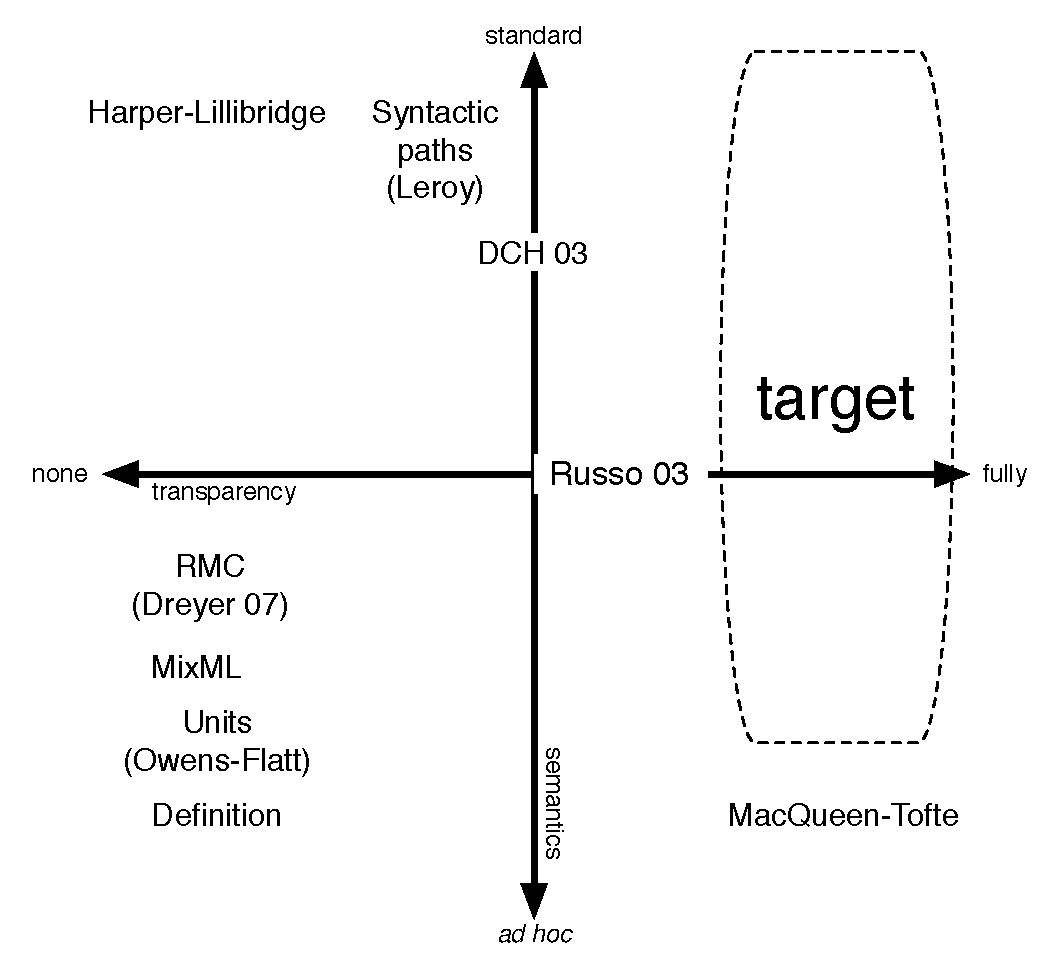
\includegraphics[scale=0.5]{../design/figs/modsys-spectrum.pdf}
\hrulefill\\
{\small A semantics is more standard in the sense that it uses more formal logic frameworks. It may potentially be easier to mechanize the metatheory of such semantics.}
\caption{The spectrum of major module system families}
\label{fig:spectrum}
\end{figure}

Besides the main module system features described earlier in this proposal, there are a number of other useful properties developed in the different module languages. The \emph{phase separation} \cite{hmm:phasedist} plays a fundamental role in ensuring that module systems can be typechecked fully at compile-time. This property is desirable, being consistent with our goal of static type safety. It says that a language, in this case a module, can be split into static and dynamic parts such that the static part does not depend on the dynamic. Some accounts of module systems respect phase distinction at the surface language level \cite{leroy95,russothesis}. Others respect the phase distinction in an internal language but not the surface language \cite{mt94}.  

The other key issue in a module system design is the existence of a \emph{principal signature} for modules. The term principal signature has been overloaded in meaning. Because of the many-to-many relationship between signatures and modules and the signature subtyping relationship, many signatures may be safely ascribed to a single structure. I will call the most precise signature for a structure (i.e., one that constrains all components of the structure with exact, most constraining types) the \emph{full signature}. A related concept is the \emph{free instantiation} of a functor formal parameter. The free instantiation is an instance of the functor formal parameter signature S that admits exactly enough type sharing to satisfy $S$ and no more. In particular, it avoids any extraneous type sharing that would cause potentially distinct types to be shared. What Dreyer \cite{dreyerthesis} calls the principal signature is the full signature in this terminology. Tofte defines principal signature of a signature expression $sigexp$ as one whose formal tycons can be instantiated to obtain all instantiations of $sigexp$ \cite{tofte92,mthm97}. I will adopt Tofte's terminology. 
   
\subsection{Syntactic Approach}
\subsubsection{CMU School}
Beginning with Harper-Lillibridge's translucent sums module calculus \cite{lillibridge94}, this large, prolific family of module systems pushed the state-of-the-art in terms of the type theoretic approach to module system design. Although Harper-Lillibridge originally explored first-class modules, the bulk of the research in this family was directed towards an applicative higher-order module semantics for type-directed compilers TIL/TILT and adding recursion. 

Crary \etal~\cite{crary99} and later Dreyer \cite{dreyer04,dreyer07} (DCH)
have explored adding support for recursion. Harper-Lillibridge
\cite{lillibridge94} and then Russo \cite{russo00} studied mechanisms
for making modules first-class entities in the core language. With
first-class modules, programmers can leverage the familiar module
system to take advantage of the System F-like power of the module
system for programming-in-the-small. Unfortunately, as Garcia
\cite{garcia05:extendedcomparing05} remarks, the syntactic overhead of
the ML module system makes this undesirable and impractical. When used
in a similar context, Garcia suggests that the type inference used for
type classes makes modular programming-in-the-small more
succinct. This observation holds only in the specialized case of type
classes. 

Harper and Stone \cite{harperstone} gave a semantics for ML modeling
every core language construct in terms of modules. This semantics was
based on the technique of using singleton signatures (and types) to
express type definitions \cite{stone00}. Dreyer's semantics uses a signature synthesis algorithm that
constructs a signature directly from a structure expression syntax
given the static environment as context. In
contrast, THO constructs a signature solely using the static environment. 

%Would this criterion apply to an example such as functor F() = struct datatype t end? 
%Why is making the distinction between generative and non-generative types at the individual spec level necessary? Wouldn't it be possible to emulate such behavior by lifting the individual type to a singleton module? 

%structure M = 
%struct
%  structure U :> sig type u end = struct type u = int end 
%   structure V :>> sig type v end = struct type v = bool end
% end

% using Dreyer's :>> weak sealing operator. 

\subsubsection{Syntactic Paths and Applicative Functors}
One of the first formal accounts of an ML-like module system is Leroy's manifest types calculus \cite{leroy94} where manifest types are definitional type specifications. The surface language for the manifest types calculus is equivalent to that of the translucent sums calculus described by Harper-Lillibridge\footnote{Definitional specs appeared in SML/NJ 0.93 a year before the Harper-Lillibridge paper appeared.}. The key observation in the manifest types calculus is that one can typecheck manifest types by comparing the rooted syntactic paths to those types which uniquely determine type identity. Thus, type equivalence is syntactic path equivalence for type constructors.  Leroy introduced the notion of applicative functors \cite{leroy95} which held types in the result of a functor application to be equivalent to corresponding types in all other results of applications of that functor to the ``same'' argument. Several designs \cite{shao99,dhc03,russothesis} have tried to incorporate both applicative and generative functors in a single calculus. Cregut \cite{CregutMacQueen94} enriched signatures with structure equalities to obtain complete syntactic signatures for separate compilation.

Leroy introduces a relatively simple approach to module system semantics that precludes shadowing of core and module bindings \cite{Leroy:generativity,leroy00}.
The semantics supports type generativity and SML90-style definitional sharing by reducing them to solving path equivalence by way of A-normalization (for functor applications) and S-normalization (a consolidation of sharing constraints by reordering). In his module system, Leroy claims that all type sharing can be rewritten in his calculus with generative datatypes and manifest types. However, Leroy's simplified module system does not include value specifications and datatype constructors both of which can constrain the order in which specifications must be written and therefore result in situations where sharing constraints cannot be in general reduced to manifest types. 

For full transparency, Leroy proved that there is a type-preserving encoding of a stratified calculus with strong sums without generativity using applicative functors\cite{leroy95}, claiming that the existence of such an encoding is a strong hint that applicative functors support full transparency. My HO apply functor example in fig.~\ref{fig:hoapplyfct} casts some doubt on this claim. As Leroy pointed out, under the strong sums model, first-class modules are at odds with phase distinction because of the typechecker would have to do arbitrary reductions\cite{leroy94}. In contrast, because the weak sum model of the manifest types calculus does not require any reductions at typecheck time regardless of the presence of first-class modules, it does not violate the phase distinction\cite{leroy94}. In the most recent paper in the manifest types series \cite{leroy00}, Leroy abstracts away most of the core language details from the manifest calculus to obtain a mostly core language independent module system. 

Although the syntactic paths approach may very well provide the simplest account of module systems, this is at the cost of some very fundamental shortcomings such as the inability to support shadowing and full transparency. Because the account's support for type sharing is incomplete, there may also be limits to how the semantics deals with the coherency issue. This dissertation will address these issues which are fundamental to the power of the ML module system. 

\subsubsection{Other ML Variants}
Shao \cite{shao:parameterizedsigsandho,shao99} defines a signature language based on gathering (and
internally factoring out) all flexible components (\ie, open 
specs unconstrained by sharing) in a higher-order type
constructor that can be applied to obtain a signature that expresses
functor body semantic actions at a later point. The resultant
signature language superficially resembles applicative
functors. However, type constructor applications in the signature
language must be on paths. Consequently, it does not support full
transparency in the general case. 

Govereau \cite{govereau:tr05} developed an alternative
semantics based on the type-theoretic approach. He claims that there
is no declaration that produces a generative type that is not
abstract, but datatype declarations could potentially be one of these
cases. One observation Govereau makes is that the static environment
must be ordered because types are dependent. Later bindings in the environment may refer to earlier bindings. The combination of applicative and generative types leads to a soundness problem similar to that found in Russo's Moscow ML system. 

The main contribution in Govereau's semantics appears to be a syntactic way to represent generativity that obviates the need for a Dreyer's effect system for managing the interaction between applicative and generative functors. The language uses distinct declarations for generative and non-generative abstract types. The type system declaratively partitions the static environment into two, corresponding to the lexical scope inside and outside a functor. 

The paper claims that if a type is defined ``under functor'' but does
not depend on a generative type defined under a functor, then it can
be coerced to non-generative. The claimed win is that although the syntactic purity judgment is not as fine-grain as DCH's effect system, it is simpler to work with. One disclosed limitation to both Govereau and Russo's systems is that a non-generative functor cannot have any generative types that are used in the body of the functor. 

Alice ML provides a number of the features mentioned in this chapter especially in the 
area of signature language enrichments. The language supports nesting signatures inside of signatures.
\begin{lstlisting} 
signature S = sig signature M = sig type t end end
\end{lstlisting}
Furthermore, the nested signatures can be left open to support signature-polymorphic functors.
\begin{lstlisting}
functor F (X:sig signature S structure Y : S end)  = ...
\end{lstlisting} 
The abstract signatures do not, however, appear to be complemented with any bounded polymorphism features. 

MLKit's semantics for elaboration calls for what amounts to defunctorization. In Elsman's view, functors are purely static constructs that can be compiled away, generating inlined copies of relevant dynamic content upon functor application. 
 
		Dreyer and Rossberg \cite{mixml} show how to encode ML signatures, structures, and functors in a mixin module calculus that appeals to something similar to Bracha's merge\cite{bracha:thesis} as its only linking mechanism. When linking a module A and B, the semantics tries to satisfy the imports of A using the exports of B and vice versa. The mixin merging syntax is {\bf link} x=M0 {\bf with} M1 in the surface language. It binds the name x to a module M0 and concatenates it with M1 merging components where appropriate. The scope of x is the body of M1. This mixin merging semantics supports recursion and separate compilation. Modules in this language consist of atomic modules that only contain values, types, type constructors, {\it etc}., labeled modules ($\{\ell = M\}$), and the merging form link ... with ....  

The peculiarity in this language is that modules and indeed anything that can be encoded in these modules are stateful. For example, signatures in MixML are fundamentally stateful. Linking against a signature S mutates it. Consequently, the typechecker rejects the following program. 
\begin{lstlisting}
module U = link x={module S = {type t}} 
           with {module A=(link x=x.S with {type t = int}), 
                 module b=(link x=x.S with {type t = bool})};		
\end{lstlisting}
Signatures must be suspended and then new'ed in order to be matched multiple times. This suspension is called a unit in Dreyer and Rossberg's terminology. Functors are also represented by suspending modules with unsatisfied imports. Although units have full support for hierarchical composition, MixML's design still retains the problem of stratifying modules and units, a problem inherited from the Flatt-Felleisen units that inspired it. 

	As it stands, the part of the MixML language that encodes the ML module system is but a small fraction of the whole. The question remains what implications the rest of the language has. Part of the language is obviously semantically meaningless such as {\bf link} X = [int] {\bf with} [3], which is a well-formed program. 

\subsubsection{Moscow ML}
Biswas gave a static semantics for a simpler form of higher-order modules \cite{biswas95}. The account relies on semantic objects and a stamp-based semantics similar to the Definition. The type propagation in higher-order functors is captured by a ``higher-order'' dependency variable that abstracted possible dependencies on the argument. These variables are only present in the internal language produced during elaboration. Consequently, Biswas's semantics does not support true separate compilation and neither does it enrich the surface syntax for signatures. Biswas's elaboration rule in fig.~\ref{fig:biswas-abstypespec-elab} maps an abstract type name t to the fresh higher-order abstract dependency variable $f$ applied to the list of all abstract dependency variables $\mathcal{W}$ it could possibly depend upon. For example, the functor parameter of the Apply functor, \lstinline{functor F(X:sig type t end): sig type t end}, is given the semantic representation $\forall f_0(\{t\mapsto f_0\} \Rightarrow \{t\mapsto f_1(f_0)\})$.

\begin{figure}
\hrule
~\\
\[
\infer {\Gamma,\mathcal{W}\vdash\mathrm{type~t}\Rightarrow ((t \mapsto f(\mathcal{W}), \emptyset), \{f\})}
{\textrm{$f$ is a fresh higher-order dependency variable}}
\]
$\Gamma$ is the type environment mapping program variables to types. $\mathcal{W}$ is a list of formal parameters variables the specification may depend on.
\hrule
\caption{Biswas's elaboration rule for abstract type specifications}
\label{fig:biswas-abstypespec-elab}
\end{figure}


Biswas's formal account was extended in a somewhat more type-theoretic
style to the full SML language and implemented by Russo in the Moscow
ML compiler \cite{russothesis}. One semantic
innovation was the use of existential types to represent abstract
types in a module system. The idea of using existential types
originated in a paper by Mitchell and
Plotkin~\cite{mitchellplotkin:popl85}. MacQueen pointed out how
scoping unpacks make conventional existential types ill-suited for
modular programming \cite{macqueen:popl86}. Montagu and R\'emy
\cite{Montagu-Remy:popl09:fzip} recently tried to address these
concerns by developing a variation of existential types which replaces
unpack with modular open and scope restriction constructs. 

Moscow ML also adds support for first-class
modules\cite{russo00} and a form of recursion \cite{russo01}. Moscow ML further attempts to incorporate both non-propagating
generative functors and applicative functors. The main limitation, as pointed out by Dreyer \cite{dreyerthesis}, is that Moscow ML's combination of generative and applicative functors is unsound. In particular, any generative functor can be $\eta$-expanded into an applicative functor thereby circumventing the generative functor abstraction. 

Russo notes the conflict between true separate compilation and
first-order module systems. He works around the problem by defining
compilation units to be only the sealed modules in an applicative
higher-order module system with first-order generative functors. To
address the avoidance problem, he introduces a hybrid name and
deBruijn-indexing scheme. 

Rossberg, Russo, and Dreyer \cite{tldi2010} developed a formal semantics based on a
translation to System F$_\omega$ enriched with records and existential
types in a recent variation on Russo's type system. In
this account, the type system of the module system was exactly the
type system of their variation on System F$_\omega$. All semantic
representations of signatures explicitly existentially quantified all
primary type constructors. The module system supported type
generativity insofar as existentials support it. The module system
does not claim to support full transparency, although there is an
extension of the system to support applicative functor semantics. 


\subsection{Units and Other Extralinguistic Linking Systems}
Flatt-Felleisen \cite{ff98} and Owens-Flatt \cite{owensflatt06} develop a module system semantics based on a calculus with stratified distinct hierarchically composable modules and recursively linkable units. Because both accounts appeal to extralinguistic linking semantics, they fall under the Module/Mesa line of module systems. As pointed out by Dreyer\cite{mixml}, the fundamental limitation in this semantics is that the stratification of units and modules precludes using unit linking and hierarchical composition together. One strength of their module system design is that it is one of the few accounts that includes an operational dynamic semantics, unlike all the other accounts discussed in this section. Some accounts of module systems give only a static semantics and perhaps a typechecking algorithm. Owens and Flatt prove type soundness of their semantics. 

Swasey \etal~\cite{swasey06} described a calculus SMLSC that is modeled after Cardelli's linkset approach to separate compilation. SMLSC introduces a compilation unit that sits on top of the module system that can be separately compiled from unimplemented dependencies by means of a handoff unit whose role resembles that of header files in C.

\subsection{The Definition and MacQueen-Tofte}
The module system semantics in the Definition of Standard ML \cite{mth90,mthm97} evolved throughout the late 1980s and early 1990s. Early on, Harper \etal~gave a fairly complete account of the static semantics of the first-order ML module system in terms of an operational stamp-based semantics \cite{hmt:tapsoft87}. Tofte in his thesis  \cite{toftethesis} proves that signature expressions in the first-order, generative semantics have principal signatures. He also extended this proof to cover non-propagating higher-order generative functors \cite{tofte:jfp94}. Then MacQueen and Tofte \cite{mt94} introduced true higher-order functor semantics. 

%Key to the semantics is the partitioning of structures into signature and {\bf realization} halves. A signature is the skeletal form of the structure, \ie, type and value specifications, with flexible type specifications that can be instantiated by signature matching. A realization fills in these flexible type specifications. 

Apart from type propagation transparency issues, the evolution of the Definition also addressed type sharing issues. The role of \emph{type sharing constraints} has evolved through the development of the Standard ML semantics and SML/NJ implementation. Type sharing constraints solve two problems in ML, type specification refinement and coherence. Originally, type specifications only declared the name of an expected type. It is quite useful to be able to refine type specifications to restrict them to particular definite types or by defining them relative to open specs. The \emph{coherence problem} is the challenge of constraining type components of two structures to be equivalent regardless of the actual identity of that type. In SML90 \cite{mth90}, explicit sharing equations among visible abstract type constructors and generative structure sharing were the sole means for constraining type specifications. Under generative structure sharing semantics, each structure had a unique static identity. Thus, two structures shared only when they were identical in the sense that they were defined at the same point in the program and are merely aliases (fig.~\ref{fig:structuresharing}). Under SML90 identity-based structure sharing, A and B have to be aliases, so the functor application at M4 fails to typecheck. Under SML97, the sharing constraint merely rewrites to sharing type A.t = B.t, thus both functor applications typecheck.
  Structures that shared in SML90 were equivalent both statically and dynamically. This kind of rich sharing semantics turned out to be quite complicated and was abandoned in favor of a structure sharing that implied type sharing constraints on congruent type specifications within the respective signatures. 

\begin{figure}
\begin{center}
\begin{tabular}{c}
\begin{lstlisting}
signature S0 = 
sig 
  type t
  val f : t -> t
  val state : t ref
end

functor F(X:sig 
           structure A : S0
           structure B : S0
           sharing A = B
          end) = ...

functor G() = 
struct
  type t = unit
  val f = ...
  val state = ref 0
end

structure M0 = G()
structure M1 = G()
structure M2 = M0

structure M3 = F(struct 
                structure A=M0
                structure B=M2
               end)

structure M4 = F(struct
                structure A=M0
                structure B=M1
               end)
\end{lstlisting}
\end{tabular}
\end{center}
\caption{SML90 structure sharing example}
\label{fig:structuresharing}
\end{figure}

SML/NJ 0.93 introduced definitional specifications, giving programmers two ways for constraining types to definite ones. SML97 added \lstinline{where type} and definitional type specifications completely replaced the definitional type sharing found in SML90. Definitional specifications and type sharing were finally disentangled. Generative structure sharing was eliminated in favor of the simpler semantics of a structural sharing that amounted to a type sharing equation for each common type component path, no matter how deeply nested. The semantics of type sharing and related mechanisms such as \lstinline{where type} are still somewhat problematical and unsettled \cite{narbel:jfp07,ramsey05}. Ramsey \etal~have argued that the scoping of \lstinline{where type} definitions should be more symmetric thereby permitting more flexible type specification refinements.

Shao \cite{shao98} (in a paper unrelated to the one on applicative functor-like module system \cite{shao99}) extends MacQueen-Tofte fully transparent modules with support for type definitions, type sharing (normalized into type definitions), and hidden module components. This treatment of higher-order modules is a more recent form of what is currently in the SML/NJ compiler. Elsman presents a module system compilation technique used in the ML Kit compiler \cite{elsman99}. The semantics follows the style of the Definition. The compilation technique is comparable to Shao's FLINT compilation scheme. 

The SML/NJ compiler implements a version of the module system that departs from the Definition in a number of aspects. Some of these extensions have not been formalized as of yet. In particular, the compiler has a richer semantics for \lstinline{include} and the elaborator compiles a functor body to a static lambda calculus which is what is used in place of the functor body re-elaboration at functor applications. The scoping of sharing constraints has also changed. In the current implementation, SML/NJ no longer permits nonlocal forms of sharing of the flavor illustrated in the example in MT (the first structure sharing constraint in fig.~\ref{fig:nonlocalsharing}). Both sides of the constraint must be in local scope as is in the second sharing constraint. Instead, structure definition specs express the same kind of sharing. For example, the structure definition spec \lstinline{structure A : sig end = S} expresses the first sharing constraint in SIG. The module system also has some significant limitations such as a lack of recursion, the tension between separate compilation and fully transparent generative functors, and weak facilities for signature composition.

\begin{figure}
\begin{center}
\begin{tabular}{c}
\begin{lstlisting}
structure S = struct type t end;
signature SIG = 
sig
  structure A : sig type t end
  structure B : sig type s end
  structure C : sig type s end
  sharing A = S
  sharing B = C
end	
\end{lstlisting}
\end{tabular}
\end{center}	
\caption{SML90-style structure sharing}
\label{fig:nonlocalsharing}
\end{figure}

\subsection{Type Generativity}

The idea of generative types has a significant history. More recently,
Neis~\emph{et al} \cite{neis:icfp09}, Dreyer and
Blume~\cite{dreyerblume:esop07}, Dreyer \cite{dreyer05}, and Rossberg
\cite{rossberg:ppdp03} have all developed semantics for studying type
generativity in the context of a System F$_\omega$-derived
language. Although the ML module system utilizes type generativity, it
only plays a role within the module system proper. After translation,
at which point the modules are eliminated, all the type generation has
already occured, having been carried out by the
elaborator. Consequently, the target language for translation, a
System F$_\omega$ language, need not contain any facilities for
generating fresh types. 

\subsection{First-class polymorphism inference and type classes}
	Jones \cite{jonesfcp} motivated first-class polymorphism (FCP) by appealing to the constructive logic tautologies for existentials, universals, and implication  \cite{jonesfcp}. The constructive logic rule $\langle w, \tau_w\rangle \rightarrow \tau' \leftrightarrow w \Rightarrow \tau_w \rightarrow \tau'$ corresponds to a translation of a module expression where types and values are coupled to System F$_\omega$ where types and values are decoupled (\emph{phase separation}) in the forward direction. More recent first-class polymorphic calculi such MLF \cite{Lebotlan-Remy/mlf-icfp} and FPH \cite{fph} add some limited type inference. Although inference in general may be undecidable, these limited inferencers still go a long way to make programming in these first-class polymorphic calculi more practical. If some of the ideas for inference for FCP calculi can be transferred over to a module calculus, one might also address the syntactic overhead of ML module systems. Adding FCP to the core introduces a certain amount of redundancy with respect to the FCP afforded by the module system. It would be useful to consider what exactly is redundant and whether that can be minimized. 
		
	Another language construct related to module systems that enjoys type inference is the type class. Type classes are a special case of modular programming where a kind of automatic deduction would be useful. Unfortunately, the scope of class instances are global. In Modular Type Classes, Dreyer \etal~ \cite{dhck07} develop semantics and a translation from type classes to a stylized use of the ML module system. 

\subsection{FLINT/Typed Cross Compilation}
The most closely related work is the formal semantics for a module
language called NRC given by
Shao~\cite{shao98}. Similar to this dissertation, NRC gives a formal semantics based on MacQueen-Tofte's
higher-order semantics. Unlike the present account, Shao's semantics
combines elaboration and translation into a single interweaving set of
judgments, whereas the present account cleanly separates them. The
separation of elaboration and translation is a conceptual
simplification and is also beneficial for more modular compiler
implementation. Also, Shao's semantics assumes a preprocessing step
that eliminates most of the interesting behavior involving coercive signature
matching. Although the NRC account alludes to the fact that the
functor body does not need to be re-elaborated at each application,
the NRC semantics does re-elaborate much like the MacQueen-Tofte
account. Finally, the NRC semantics does not directly support
datatype declarations, though it is claimed that it is a
straightforward extension. 

The account of NRC makes a few arguable
simplifying assumptions. Value components is a trivial extension that only requires a
  conversion of source-level types to semantic types. 
 Signature extraction is trivial only requiring the conversion of
  semantic types back to syntactic types. This conversion is
  guaranteed by the 1-to-1 mapping of the stamp environment. This is
  similar to our entity environment (see chapter~\ref{ch:entitycalc}), but as the semantics in 
  demonstrate, this is far from trivial.
 Shao says that value components in NRC are only elaborated once,
  but any type components may be re-elaborated. We simplify this even
  further. Only functor applications and type generation have to be
  re-elaborated. Type definitions can be expanded out early on during
  elaboration.
 As with some other accounts, NRC entangles type-checking and
  translation into F$_\omega$. Although translation clearly depends on
  type-checking, the converse case is not true. 
 In NRC, the assumption is that type-sharing constraints can all
  be converted to type definitions. As I have shown earlier, this is
  technically incorrect but probably practically adequate. 
 NRC requires A-normalization of the surface syntax SFC so that
  the only functor applications are of a functor variable (not
  paths) to a structure variable. In THO, the operator position of
  applications can be a path and the operand can be any structure
  expression. 
 The $\alpha$-renaming scheme described in NRC adds new
  declarations inside of existing structures in order to deal with
  signature ascription. 
 Signature matching is mostly handled during the SFC to NRC
  translation by adding explicit enrichment coercions. 
 NRC relies on a stamp environment, a finite map from stamp to
  tycon path. This has turned out to be unnecessary due to the
  existence of a function to perform the equivalent operation while
  relying on only the present semantics' structure entity itself. This function is the moral
  equivalent of an inversion of the realization although the
  realization does not technically admit an inversion. 


\subsection{Summary}
Not all module system designs enjoy the principal signature and phase distinction properties.  Fig.~\ref{fig:sys-features} summarizes the key features of the main ML-like module system families. Note that many module systems have various combinations of these features, but none are complete. Ideally, a module system would have true higher-order semantics and all the other features except for applicative functors which would be redundant. 

\begin{figure}
	\small
\begin{tabular}{|l|l|l|l|l|l|l|l|}
	\hline
System & higher-order & first-class & sep comp & rec & app & gen & phase\\
	\hline
	HL \cite{lillibridge94} & \ex & \chk & \chk & \ex & \ex & \ex & \chk \\
	\hline
	Leroy \cite{leroy95} & \ex & \ex & \chk & \ex & \chk & \ex & \chk \\
	\hline
	Russo \cite{russo01} & \ex & \chk & \chk & \chk & \chk & \chk & \chk \\
	\hline
	DCH \cite{dhc03} & \ex & \chk & \ex & \ex & \chk & \chk & \chk \\
	\hline
	RMC \cite{dreyer07} & \ex & \ex & \ex & \chk & \ex & \chk & \chk\\
	\hline
	%$\lambda^{\llparenthesis~\rrparenthesis}$ (\cite{ATTAPL}) & & & & & & \\
	%\hline
	%$\lambda^S$ (\cite{ATTAPL}) & & N & & N & N & N \\
	%\hline
	MT \cite{mt94} & \chk & \ex & \ex & \ex & \ex & \chk & \chk \\
	\hline
	MixML \cite{mixml} & \ex & \chk & \chk & \chk & \ex & \chk & \ex \\
	\hline
	Ideal & \chk & \chk & \chk & \chk & \ex & \chk & \chk \\
	\hline
\end{tabular}\\
higher-order = true higher-order\\
rec = recursive modules\\
app = applicative functors\\
gen = non-propagating generative functors\\
phase = respects the phase distinction
\caption{A comparison of major ML-like module systems}
\label{fig:sys-features}
\end{figure}		 										
 
%%% Local Variables: 
%%% mode: latex
%%% TeX-master: "main"
%%% End: 
